\documentclass[a4paper, 12pt]{article}

%\usepackage[T2A]{fontenc}
\usepackage[utf8]{inputenc}
\usepackage[normalem]{ulem}

\usepackage[english, russian]{babel}
\usepackage{amssymb, amsfonts, amsmath, mathtext, cite, enumerate, float, physics}
\usepackage{graphicx}
\usepackage{indentfirst}
\usepackage{multirow}
\usepackage{textalpha}
\usepackage{listings}

\usepackage{geometry}
\geometry{left = 2.5cm, right = 2.5cm, top = 3cm, bottom = 3cm}
\linespread{1.5}

\usepackage{xcolor} 
\definecolor{codegreen}{rgb}{0,0.6,0}
\definecolor{codegray}{rgb}{0.5,0.5,0.5}
\definecolor{codepurple}{rgb}{0.58,0,0.82}
\definecolor{backcolour}{rgb}{0.95,0.95,0.92}
 
\lstdefinestyle{mystyle}{
    backgroundcolor=\color{backcolour},   
    commentstyle=\color{codegreen},
    keywordstyle=\color{magenta},
    numberstyle=\tiny\color{codegray},
    stringstyle=\color{codepurple},
    basicstyle=\ttfamily\footnotesize,
    breakatwhitespace=false,         
    breaklines=true,                 
    captionpos=b,                    
    keepspaces=true,                 
    numbers=left,                    
    numbersep=5pt,                  
    showspaces=false,                
    showstringspaces=false,
    showtabs=false,                  
    tabsize=4
}

\lstset{style=mystyle}


\usepackage{fancyhdr}
\pagestyle{fancy}
\rhead{Кусайко Г.Н.}

\graphicspath{ {images/} }

\begin{document}
    \begin{titlepage}
    \begin{center}
        МИНИСТЕРСТВО НАУКИ И ВЫСШЕГО ОБРАЗОВАНИЯ\\
        РОССИЙСКОЙ ФЕДЕРАЦИИ\\
        Федеральное государственное автономное образовательное учреждение\\
        высшего образования\\
        <<ТЮМЕНСКИЙ ГОСУДАРСТВЕННЫЙ УНИВЕРСИТЕТ>>\\
        ИНСТИТУТ МАТЕМАТИКИ И КОМПЬЮТЕРНЫХ НАУК\\
        Кафедра фундаментальной математики и механики
    \end{center}

    \vspace{8em}

    \begin{center}
        ОТЧЕТ ПО НАУЧНО-ИССЛЕДОВАТЕЛЬСКОЙ РАБОТЕ
    \end{center}

    \vspace{6em}

    \begin{flushleft}
        Выполнил работу \hfill Кусайко \\
        Студент 1 курса, \hfill Георгий \\
        аспирантуры \hfill Николаевич \\
        очной формы обучения \\
        \vspace{1.5em}
        Руководитель работы \hfill Игошин \\
        к.ф.-м.н., ? \hfill Дмитрий \\
        \hfill Евгеньевич \\
    \end{flushleft}
    
    \vspace{\fill}

    \begin{center}
        Тюмень, 2021
    \end{center}
\end{titlepage}


    \tableofcontents
    \newpage

    \section{Введение}
    На момент написания отчета были сформулированы следующие цели и задачи:
    \begin{itemize}
        \item подбор необходимой литературы и документации;
        \item изучение следующих вычислительных программных пакетов и утилит:
        \begin{itemize}
            \item SALOME;
            \item OpenFOAM;
            \item Paraview.
        \end{itemize}
        \item автоматизация вычислительного процесса, а также использование параллельных вычислений.
    \end{itemize}
    \newpage

    \section{Процесс вычисления}
    Обычно, моделирование и процесс вычисления происходит последовательно по следующим этапам:
    \begin{enumerate}
        \item \textbf{Подготовительный этап}. На данном этапе формируется геометрия модели, формулируются необходимые физические условия, геометрия дискретизируется, задаются начальные и граничные условия дифференциальных уравнений;
        \item \textbf{Расчёт}. На данном этапе машина, подчиняясь заданному алгоритму, численно решает основные уравнения с точки зрения базовых физических параметров (скорость, давление, плотность, температура, энтальпия и т. д.), а также записывает результаты решения в память;
        \item \textbf{Постобработка}. Выполняется конвертация результатов расчёта в форматы, пригодные для отображения и визуализации.
        \item \textbf{Анализ}. Результаты решения отображаются в виде графиков, таблиц, а также контурных или векторных схем, привязанных к исходной геометрии.
    \end{enumerate}

    На этих этапах чаще всего используется не один, а сразу ряд инструментов. Такой подход и будет рассматриваться в дальнейшем.

    \section{Подготовительный этап}
    В качестве модели возьмем модифицированную объемно-центрированную кубическую решетку. Радиус зерен (сфер) будет
    \[
        R = \frac{1}{1 - \alpha},
    \]
    где $\alpha$ - параметр, определяющий пересечение зерен. Т.е. при $\alpha = 0$ они не будут пересекаться, но будут соприкасаться. Размер самой структуры
    \[
        \Delta x = 2 \sqrt 2, \Delta y = 2 \sqrt 2, \Delta z = 2.
    \]
    
    Построение геометрии, а также дискретизацию будем проводить в программном пакете SALOME. Данный пакет обладает обширным функционалом, а рабочий процесс обычно производится через графический интерфейс. Однако почти все подключаемые модули написаны на языке программирования Python. Это дает возможность для написания исполняемых скриптов, которые можно запускать из командной строки. Для этого требуется запустить сессию сервера SALOME и передать туда скрипт. 
    
    Недостатком же SALOME, является то, что запущенная сессия может работать только на одном ядре процессора, т.е. если потребуется построить несколько структур с отличающими параметрами и дискретизировать их за один раз, это будет исполнено последовательно, что сильно скажется на затраченном времени. Таким образом, приходим к тому, что необходимо распараллелить последовательность вычислений для разных параметров. В данном случае это будет параметр $\alpha$.

    Для решения данного момента используем стандартную библиотеку Python, которая называется multiprocessing. Также, чтобы инициализировать сессию SALOME и передать туда исполняемый скрипт, потребуется библиотека subprocess. 

    \lstinputlisting[language=Python, caption={genmesh.py}]{src/genmesh.py}

    Как мы можем видеть на Листинге 1, происходят следующее важные шаги:
    \begin{enumerate}
        \item Подключаем необходимые библиотеки;
        \item Задаем параметр $\alpha$, а также структуры, которые необходимо просчитать (в данном случае одну);
        \item Создаем функцию, через которую будем запускать сессиию SALOME с необходимыми аргументами.
        \item Инициализируем процесс для каждой структуры, а также для каждого параметра $\alpha$, которые будут выполняться параллельно, в зависимости от количества ядер процессора, а также их занятости.
    \end{enumerate}

    Также можно заметить, что был использован скрипт <simple-cubic/main.py>, в котором как раз и содержится построение геометрии модели и ее дискретизация. Это файл тут не будет прикладываться, так как он объемный и разбит на несколько логических модулей.
    
    \begin{figure}[t!]
        \centering
        
        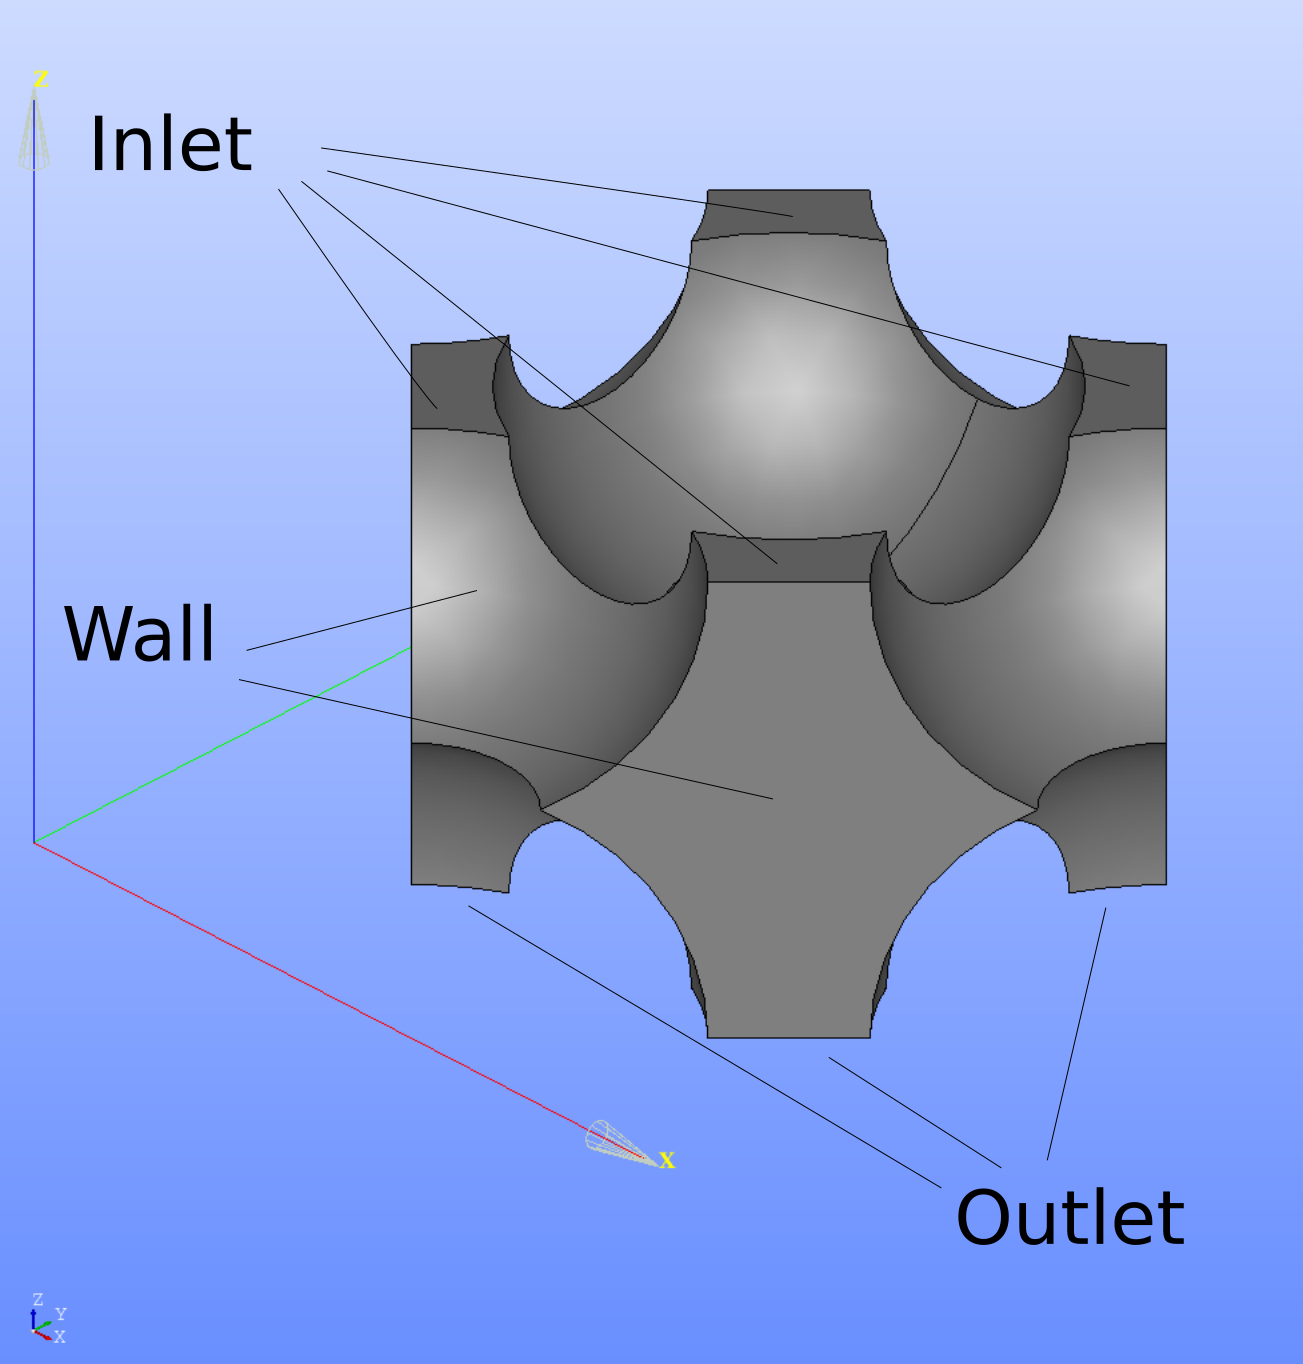
\includegraphics[scale=0.2]{simple-cubic}
        \caption{ASD}
    \end{figure}

    Стоит упомянуть, что полученные поверхности геометрии структуры были сгруппированы как inlet, outlet и wall, т.е. поверхности для входящего потока, выходящего и стенок соответственно. Это шаг необходим для задания начальных и граничных условий в OpenFOAM. Так как мы задаем однофазный поток, направленный вертикально вниз, то получаем группы, которые изображены на Рис. 1. Граничные и начальные условия:
    \[
        wall: \vec{v} = 0, \frac{d p}{d n} = 0;
    \]
    \[
        p_{inlet} = 1 \text{Па};
    \]
    \[
        p_{outlet} = 0;
    \]
    \[
        \vec{v}(x, y, z) = 0.
    \]
    Численное решение уравнений
    \[
        \nabla \cdot \vec{v} = 0,
    \]
    \[
        \nabla \cdot (\vec{v} \vec{v}) - \nu \Delta \vec{v} = -\frac{1}{\rho} \nabla p,
    \]
    будет осуществляться с помощью решателя SIMPLE.
    \newpage

    \section{Расчёт}
    После дискретизации геометрии получаем на выходе файл формата UNV, который содержит информацию по сетке, а также по группам, необходимым для начальных и граничных условий. В силу небольшой специфики OpenFOAM, нужно создать директорию, где и будут находиться файлы, необходимые для расчёта.

    \lstinputlisting[language=sh, caption={tree simple-cubic/0}]{src/simple-cubic-tree}

    Для импортирования сетки из формата UNV в формат, понятный для OpenFOAM, используется утилита ideasUnvFoam. После ее применения появляется директория constant/polyMesh, в которой необходимо изменить в файле boundary значение для группы wall на wall, так как стандартно после импортирования для всех групп задается значение patch.

    Таким образом, мы подготовили все к расчету, остался только момент с параллельными вычислениями. OpenFOAM изначально их поддерживает, а реализация осуществляется через OpenMPI. Однако чтобы запустить, требуется сначала выполнить декомпозицю текущей директории с помощью decomposePar. Настройки для данной утилиты задаются в system/decomposeParDict cоответственно. Допустим, у нас есть 4 ядра процессора, которые можем использовать для расчета, тогда после выполнения получим на выходе 4 связанные директории processor0 - processor3 (индексация с нуля), в которых будут содержаться измененные файлы с начальными и граничными условиями 0/U и 0/p, а также constant/.

    Далее остается только запустить расчёт, попутно записывая стандартный вывод утилиты в файл simpleFoam.log (см. Листинг 3).

    \begin{lstlisting}[language=sh, caption={sh}]
$ mpirun -np 4 simpleFoam -parallel | tee simpleFoam.log
    \end{lstlisting}

    Результируя, получаем следующий bash-скрипт, который автоматизирует процесс запуска вычислений для каждого параметра $\alpha$ (см. Листинг 4).

    \lstinputlisting[language=sh, caption={compute.bash}]{src/compute.bash}
    \newpage

    \section{Анализ результатов}
    Визуализация будет проводиться с помощью программного пакета ParaView. Данный пакет также имеет широкий функционал, позволяющий отображать не только объемные фигуры и строить графики, но и проводить дополнительные манипуляции с объектами, например, срезы, отображение полей для полученных физический величин.
    Однако этот этап процесса вычисления не будет приведен в данном отчете по следующим причинам:
    \begin{enumerate}
        \item Требуется доработка, связанная со сходимостью решения. Необходима автоматизация корректировки параметров влияющих на это, например, коэффициентов релаксации и др.
        \item Расчёт ведется еще для нескольких структур. Финальные результаты всей работы будут оформлены в статье, поэтому данные не раскрыты, а параметры упомянутые выше выбраны условно.
    \end{enumerate}
    \newpage

    \section{Выводы}
    \newpage

    \section{Список литературы}
\end{document}
